\documentclass{standalone}
\usepackage{tikz}
\usepackage{graphicx}

\usepackage{pgfplots}
\pgfplotsset{compat=1.18}
\usepgfplotslibrary{fillbetween} % Required library

\usetikzlibrary{decorations.pathmorphing}

\usetikzlibrary{calc}


% Define the precise pixel mapping factor for 96 DPI
% (72.27 points per inch / 96 pixels per inch)
\newcommand{\px}{0.75281pt}


\newcommand*\circled[4]{\tikz[baseline=(char.base)]{
    \node[shape=circle, text=#2, fill=#3, draw=#4,
     text opacity=1, fill opacity=1, draw opacity=1,  
     inner sep=2pt, minimum size=0pt] (char) {#1};}}

\makeatletter
\newcommand{\empolygon@impl}[2]{%
 \draw[red, thick, fill=red!20, fill opacity=0] (em#1-1) 
    \foreach \i in {2,...,#2} { -- (em#1-\i) } -- cycle;

 \node (em#1-node) at (em#1-1) [anchor=north west, %xshift=-5pt, yshift=-5pt, 
  draw=yellow, draw opacity=.4, fill=yellow, fill opacity=.1] {\circled{#1}{black}{white}{yellow}};
}

\newcommand{\empolygon}[1]{%
\empolygon@impl{#1}{\@nameuse{em#1-count}}
}
\makeatother


\tikzset{
 legalpaper/.pic={
   \coordinate (c1) at (0, 0);
   \coordinate (c2) at (30, 0);
   \foreach \i in {1,2,...,27} {
     \draw[blue!30, ultra thin] ($(c1)+(0,-\i*\px)$) -- ($(c2)+(0,-\i*\px)$);
  }
 }
}


\tikzset{
 legalpaperimg/.pic={
   \node at (0,0) [anchor=north west] {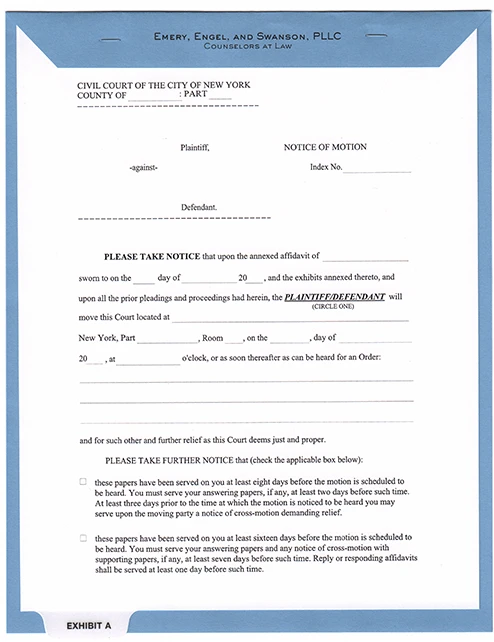
\includegraphics[width=30pt]{p.png}};
   \coordinate (c1) at (9, 3);
   \coordinate (c2) at (36, 3);
   \foreach \i in {1,2,...,27} {
     \draw[blue!30, ultra thin] ($(c1)+(0,-\i*2*\px)$) -- ($(c2)+(0,-\i*2*\px)$);
  }
 }
}

\tikzset{
 starsix/.pic={
   \draw[thick] %, decorate, decoration={random steps, segment length=2mm, amplitude=0.5mm}] 
    (90:12)  to [bend left=-5] (210:12) to [bend left=-5] (330:12) to [bend left=-5] cycle;
  
   % Downward-pointing triangle (vertices at 270°, 30°, 150°)
   \draw[thick] % , decorate, decoration={random steps, segment length=2mm, amplitude=0.5mm}]
    (270:12) to [bend left=-5] (30:12) to [bend left=-5] (150:12) to [bend left=-5] cycle;
 }
}


\tikzset{
  % This style forces the path picture content to match the node's dimensions
  expand to shape/.style={
    path picture={
      \fill[#1] (path picture bounding box.south west) 
      rectangle (path picture bounding box.north east);
    }
  }
}


  % Define the reusable curve path macro
  \newcommand{\mycurve}{(0,0) .. controls (10,20) and (20,-10) .. (40,10)}



\begin{document}
\begin{tikzpicture}[x=\px, y=-\px, every node/.style={transform shape}]% x=1pt, y=-1pt] 

\fill[lightgray] (0,0) rectangle (500,800);

\useasboundingbox (0,0) rectangle (500,800);

%\node[anchor=south west, inner sep=0, outer sep=0] (image) at (0,0) 
%   {\includegraphics[width=512pt]{i.png}};

%\begin{scope}[xscale=1,yscale=1,xshift=0,yshift=512pt]


\begin{scope}[xshift=140, yshift=-140, xscale=5, yscale=5]

 \pic [xslant=0.2, yslant=0.1, rotate=-10] 
   at (0, 0) {starsix};

% \pic [cm={1.0, 0.3, 0.5, 1.2, (0, 0)}] at (0, 0) {starsix};

%   \draw[thick] %, decorate, decoration={random steps, segment length=2mm, amplitude=0.5mm}] 
%    (90:12) -- (210:12) -- (330:12) -- cycle;
  
   % Downward-pointing triangle (vertices at 270°, 30°, 150°)
%   \draw[thick] % , decorate, decoration={random steps, segment length=2mm, amplitude=0.5mm}]
 %   (270:12) -- (30:12) -- (150:12) -- cycle;


\end{scope}


  \pic at (40,40) {legalpaperimg};
  \pic[scale=1.5] at (70,70) {legalpaperimg};
  \pic[rotate=45] at (110,110) {legalpaperimg};


\coordinate (c1) at (11, 3);
\coordinate (c2) at (31, 3);


% \foreach \i in {1,2,...,27} {
%    \draw[blue!30, ultra thin] ($(c1)+(0,-\i*\px)$) -- ($(c2)+(0,-\i*\px)$);
%  }
  
  % Optional: Draw a vertical red margin line
  % \draw[red!60!white, thick] ($(current page.north west)+(1.5cm,0)$) -- ($(current page.south west)+(1.5cm,0)$);



\begin{scope}[xscale=1,yscale=1,xshift=0,yshift=512pt]

 % pattern is  \coordinate (em#-#) at (x, y);

\coordinate (em1-1) at (171, 376);
\coordinate (em1-2) at (172, 375);

\end{scope}


\draw [
  thick,
  path picture={{
    \node at (path picture bounding box.center) [expand to shape=orange!30] {
      \tikz \pic {legalpaperimg};
    };
  }}
] (350,350) circle (12pt);



\begin{scope}[xshift=100, yshift=-290]

\draw[green!50!black,thick,name path=A]  \mycurve{} ; % arc [start angle=180,   end angle=360];
\draw[red,thick,name path=B, yshift=-30]   \mycurve{} ; %(100,600) arc [start angle=180,   end angle=360];
\tikzfillbetween[of=A and B]{blue, opacity=0.2};

\end{scope}


\begin{scope}[xshift=190, yshift=-190]

  % Combine the curves into a single filled/drawn shape
  \draw[draw=orange!80!black, thick, name=ctop]
    \mycurve{} ;      

  \draw[draw=orange!80!black, thick, yshift=20pt, name=cbot]
    \mycurve{} ;      


 \begin{scope}


   \addplot[name path=fill, draw=none] fill between[of=ctop and cbot];

   \clip [pgfplotsclipnotext] [on layer=axis background] \pgfextra{\pgfplotspathfillbetween};

   \node[anchor=south west] at (axis cs:0,0) {
            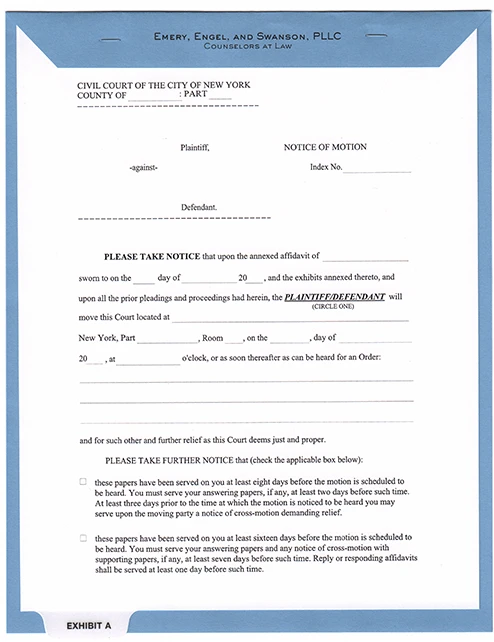
\includegraphics[width=5cm, height=5cm]{p.png}
        };

    \end{scope}

   %\fill [orange!30] fill between[of=ctop and cbot];

%  \tikzfillbetween[of=ctop and cbot]{blue, opacity=0.2};


% Source - https://tex.stackexchange.com/a/381611
% Posted by Bobyandbob
% Retrieved 2026-10-21, License - CC BY-SA 3.0




%\begin{scope}
        % Clip a closed region using Path A and a bounding box underneath
%        \clip \pathA -- (130,-200) -- (0,-200) -- cycle;
        % Fill a closed region using Path B and a bounding box above
%        \fill[blue!20] \pathB -- (300,200) -- (0,200) -- cycle;
  
%  \end{scope}


                  % Draws the first copy
%    -- ([yshift=-1cm]40,10)                % Line down to the start of the second curve
%    [shift={(0,-1cm)}] \mycurve % Second curve in reverse (shifted down)
%    -- cycle;                            % Closes the shape back to the start


\end{scope}


\end{tikzpicture}
\end{document}


